\section{Research Idea 5: Explicit Geometry and Human Pose for Social-Norm Reasoning}
\subsection{Initial Implementation}
\label{sec:idea5-impl}

We report EgoNormia~\citep{rezaei2025egonormia} joint accuracy (action and justification both correct) on the 200 verified items $T$, where ``None of these'' is never correct, and use 600 items from disjoint videos for training and cross-validation. Since explicit depth can improve spatial reasoning~\citep{cheng2024spatialrgpt}, each item's five-frame RGB strip is also rendered as depth (Depth-Anything-V2-Small), instance-segmentation (YOLOv8n-seg) and body/hand-skeleton (MediaPipe) maps, each described by Gemini~4 without seeing the question; the same extractors give four spatial labels (people count, nearest distance, facing, hands visible). Every spatial condition is paired with a matched control carrying the same amount of non-spatial input (mismatched maps and descriptions, repeated RGB, a non-spatial description, or a LoRA trained on non-spatial data), and we call the difference a spatial-specific effect.

\paragraph{Universal embedding and direct answering.}
First, a frozen Qwen3-VL-Embedding-8B model encodes the context into $\mathbf c$ and each option into $\mathbf o$ across four conditions: RGB plus description (C2), C2 plus visual maps and their descriptions (C5), C5 with mismatched maps and descriptions (X1), and C2 with repeated RGB (X3). Over these vectors, we fit a low-rank bilinear scorer with an option prior and abstention bias,
\begin{equation}
s(\mathbf c,\mathbf o)=\alpha\,\mathbf c^{\top}\mathbf o+(A\mathbf c)^{\top}(B\mathbf o)+\mathbf v^{\top}\mathbf o+\beta\,\mathbf 1[o=\text{None}],
\end{equation}
which we train using softmax cross-entropy over the options $O^{h}_i$ of each head $h\in\{a,j\}$,
\begin{equation}
\begin{split}
\mathcal L_{\mathrm{sc}}={}&-\tfrac1N\textstyle\sum_{i}\sum_{h}\log p\big(y^{h}_i\mid\mathbf c_i,O^{h}_i\big)\\
&+\lambda\big(\|A\|_F^2+\|B\|_F^2+\|\mathbf v\|^2\big).
\end{split}
\end{equation}
We evaluate this scorer with 5-fold video-grouped cross-validation across all 800 items and on $T$, and fit a logistic probe on $\mathbf c$ to predict the four spatial labels. In parallel, we evaluate Gemini~4, GPT-5.6, and Qwen3-VL-32B~\citep{bai2025qwen3vl} in zero-shot answering on RGB alone, visual maps, mismatched maps, repeated RGB, and text descriptions, as well as text-only descriptions with spatial relations reworded or reversed, spatial versus generic chain-of-thought prompting, and forced choice without ``None.''

\paragraph{Spatial fine-tuning and evaluation.}
To test whether learning spatial tasks transfers to social norms, we fine-tune Qwen3-VL-8B with LoRA ($r{=}16$) using $\mathcal L_{\mathrm{SFT}}=-\sum_{t\in\mathrm{ans}}\log\pi_\theta(y_t\mid x,y_{<t})$ on 5,000 spatial QA items from SAT, matched against a LoRA trained on 5,000 non-spatial VQAv2 items. We also compare four published spatial checkpoints against their base models: SpatialLadder-3B and MindCube-RL-3B on Qwen2.5-VL-3B, and SpaceR-7B and Spatial-SSRL-7B on Qwen2.5-VL-7B. Contrasts are paired by item using exact McNemar tests and 95\% bootstrap confidence intervals, pooling ten primary spatial-specific contrasts via DerSimonian--Laird random effects.

\subsection{Results and Discussion}
\label{sec:idea5-results}

Across all experiments, no spatial intervention improved social-norm accuracy beyond its matched control. As shown in Table~\ref{tab:idea5-contrasts} and Figure~\ref{fig:forest}, the pooled spatial-specific effect across all ten contrasts is $+0.2\ [-1.7,+2.1]$ percentage points (pp). Spatial fine-tuning hurts instead of helping: our SAT LoRA scores $6.5$ pp below its VQAv2 control ($-6.5\ [-12.0,-1.0]$). Spatial cues only help in the text-only baseline without images, where keeping spatial words intact beats reversing them by $+3.5\ [+0.9,+6.0]$ pp.

\begin{table}[t]
\caption{Key contrasts on EgoNormia joint accuracy ($\Delta$ in pp, 95\% bootstrap CI, exact McNemar $p$ where reported).}
\label{tab:idea5-contrasts}
\centering
\small
\setlength{\tabcolsep}{2pt}
\begin{tabular}{@{}lr@{\;}lr@{}}
\toprule
Contrast & \multicolumn{2}{l}{$\Delta$ [95\% CI]} & $p$ \\
\midrule
\multicolumn{4}{@{}l}{\textit{Embedding scorer (CV, $n{=}799$)}} \\
C5 $-$ C2 & $+2.6$ & $[+0.4,+4.9]$ & \\
C5 $-$ X1 (mismatched) & $+1.3$ & $[-0.9,+3.4]$ & \\
\multicolumn{4}{@{}l}{\textit{Direct answering (3 models pooled)}} \\
Maps $-$ mismatched maps & $-0.7$ & $[-3.2,+1.8]$ & \\
Maps $-$ RGB repeated & $+2.8$ & $[+0.3,+5.2]$ & \\
Text: reworded $-$ reversed & $+3.5$ & $[+0.9,+6.0]$ & \\
\multicolumn{4}{@{}l}{\textit{Spatial training}} \\
SAT LoRA $-$ control LoRA & $-6.5$ & $[-12.0,-1.0]$ & \\
SpatialLadder-3B $-$ base & $-12.0$ & $[-19.5,-4.5]$ & .003 \\
SAT LoRA+maps $-$ base & $-9.8$ & $[-16.5,-3.2]$ & ${<}.001$ \\
\midrule
All spatial-specific ($k{=}10$) & $+0.2$ & $[-1.7,+2.1]$ & \\
\bottomrule
\end{tabular}
\end{table}

\begin{figure}[t]
\centering
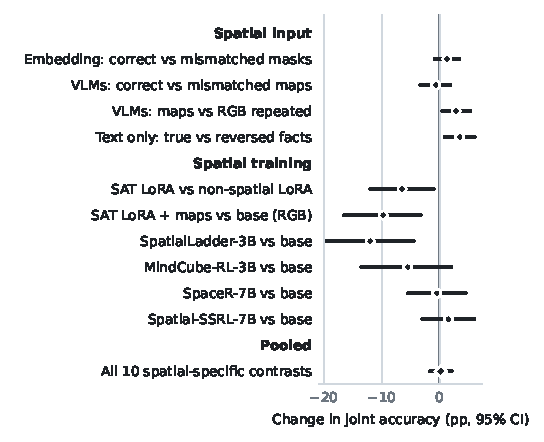
\includegraphics[width=\columnwidth]{forest_compact}
\caption{Change in EgoNormia joint accuracy (pp, 95\% CI) across spatial input and spatial training interventions, with the pooled spatial-specific effect over ten contrasts at bottom.}
\label{fig:forest}
\end{figure}

Adding the maps to the embedding (C5 vs.\ C2) raises probe accuracy by $+3.4\ [+2.2,+4.7]$ pp, so the geometry is encoded. However, while C5 improves social accuracy over C2 by $+2.6\ [+0.4,+4.9]$ pp, it does not reliably beat the mismatched-map control X1 ($+1.3\ [-0.9,+3.4]$ pp). Direct answering shows the same pattern: visual maps improve raw accuracy over RGB alone by 4 to 6 pp across the three models, but mismatched maps from unrelated videos perform equally well ($-0.7\ [-3.2,+1.8]$ pp pooled). Spatial chain-of-thought is no better than generic reasoning, and items rated as requiring high spatial understanding show no benefit ($-1.4\ [-4.6,+1.9]$ pp).

Spatial training produces an even clearer negative result. Our SAT LoRA improves held-out SAT accuracy from 78.8\% to 88.8\%, yet it falls $6.5$ pp behind the non-spatial control LoRA on EgoNormia. Published spatial models follow the same trend relative to their base checkpoints: SpatialLadder-3B changes by $-12.0\ [-19.5,-4.5]$ pp and MindCube-RL-3B by $-5.5$ pp, while SpaceR-7B ($-0.5$ pp) and Spatial-SSRL-7B ($+1.5$ pp) show little change, with larger reported spatial gains aligning with larger social losses. Combining our SAT LoRA with test-time spatial maps reduces accuracy by $9.8$ pp relative to base Qwen3-VL-8B on RGB alone, as the penalties from the adapter and the complex input simply add together without interaction. This echoes Cambrian-S, where spatial supervision reduced general video performance unless mixed with general data~\citep{yang2025cambrians}.

Inspecting model predictions reveals that most differences between input conditions reflect shifts in abstention rather than social reasoning. Adding EgoNormia's own non-spatial scene description costs GPT-5.6 9 pp, entirely through extra ``None'' picks, and a mismatched description costs Qwen3-VL-32B 22 pp, whereas mismatched maps are largely ignored. When we remove ``None'' to force a substantive choice, accuracy across conditions converges (e.g., to 71.5--73.0\% for GPT-5.6), and Gemini~4's apparent gain from visual maps comes from picking ``None'' less often. Classifying wrong predictions with a GPT-5.6 judge (checked by Gemini~4) shows that only about one in 63 to 87 errors per model involves spatial geometry; roughly 60\% stem from basic perception failures and 20--31\% reflect misjudged social norms.

As supplementary context, Figure~\ref{fig:litscaling} shows the general trend across published models. We compiled these scores ourselves from public leaderboards, so the figure describes models in general rather than a finding from prior work: for the ten models reported on both the OpenCompass spatial leaderboard and the EgoNormia leaderboard, models with higher spatial scores tend to score higher on EgoNormia as well. This is what one expects when newer and larger models improve across the board, and the spatial scores closely track general ability as measured by MMMU. Capable models are good at both, but our experiments show that pushing spatial ability on its own does not make a model better at social reasoning. Although, our experiments are conducted on exponentially smaller models and data perhaps scale could alter these findings.

\begin{figure}[t]
\centering
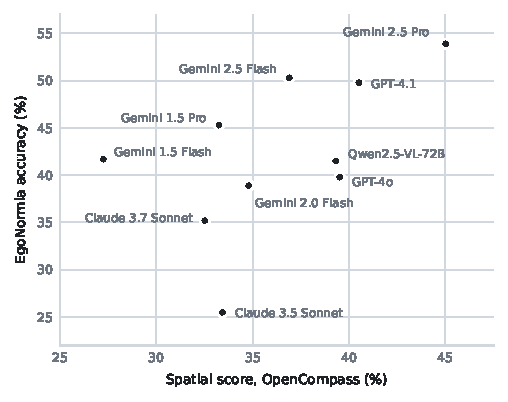
\includegraphics[width=\columnwidth]{frontier_spatial_social}
\caption{Published scores for the ten models reported in both sources: spatial score (mean of BLINK, 3DSRBench, MMSI-Bench and LEGO-Puzzles under circular evaluation; OpenCompass spatial leaderboard, 15 Aug 2025 snapshot) against EgoNormia joint accuracy (EgoNormia paper, Table~5, video models, full split).}
\label{fig:litscaling}
\end{figure}

\subsection{Updated Research Idea}
\label{sec:idea5-updated}

Our results suggest that improving a vision-language model's spatial ability does not improve, and can even degrade, its social-norm reasoning. Because this rests on one social benchmark, one spatial training set and a handful of models, we will test it across model scale (1B to 72B), family (Qwen-VL, InternVL, LLaVA-OneVision, Gemma), adaptation method (LoRA, full fine-tuning, published checkpoints) and spatial training data (static QA, synthetic 3D scenes, depth and distance QA, egocentric video, and human pose from an encoder such as Meta's Sapiens2). Each spatial run is paired with a matched non-spatial control, counts only if it improves held-out spatial benchmarks, and is evaluated on several social benchmarks (EgoNormia, SIV-Bench, MuMA-ToM, MMToM-QA, EmoBench-M, Social-IQ~2.0~\citep{siq2}), with and without the ``None'' option.

Since the aim is to show that an effect is absent, we will use equivalence tests rather than significance tests, with sample sizes fixed in advance so that small effects would be detected, and we will check whether runs with larger spatial gains also show larger social gains. The claim would be overturned by a verified spatial fine-tune that reliably improves social accuracy across seeds and benchmarks, or by a clear positive link between spatial and social gains.
